\documentclass{beamer}

\usepackage{mjclectureslides}
\usepackage{cancel}

\definecolor{Dblue}{rgb}{.255,.41,.884}

\title[Differentiation]
{Introduction to Analysis: \\ Differentiation}
%\author[Prof. Michael Carlisle]{Prof. Michael Carlisle} 
%\institute{Baruch College, CUNY}
%\date{Fall 2017}
\date{}


\begin{document}

\frame{\titlepage}

\frame{ \frametitle{Difference Quotient of a Real-Valued Function}

\begin{defn}
Let $f: (a,b) \to \R$ be a function, and $c \in (a,b)$. 

\vspace{5mm}

The \textbf{difference quotient} $D_f(x, c)$ of $f$ between $x$ and $c$ is defined as the ratio 

\[ D_f(x, c) = \frac{f(x) - f(c)}{x - c} \]

\vspace{3mm}

for any $x \in (a,b)$, $x \neq c$. 
\end{defn}

}

\frame{ \frametitle{Difference Quotient of a Real-Valued Function}

The difference quotient is the slope of the secant line between the two points $(x, f(x))$ and $(c, f(c))$ on the graph of $f$. 

\vspace{5mm}

It represents an \emph{average rate of change} of the function $f$ between the points $x$ and $c$. 

\begin{figure}[!ht]
  \centering
    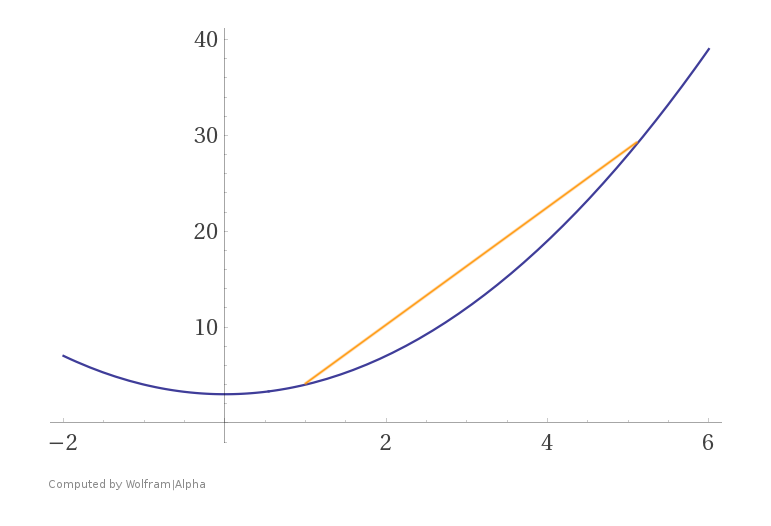
\includegraphics[width=2.5in]{WolframAlpha-yx21secant15.png}
    \caption{$f(x) = x^2 + 1$, with secant line on $f$ from $x=1$ to $x=5$}
\end{figure}

}


\frame{ \frametitle{Derivative of a Real-Valued Function}

\begin{defn}
Let $f: (a,b) \to \R$ be a function, and $c \in (a,b)$. 

\vspace{5mm}

The limit, if it exists, of the difference quotient $D_f(x, c)$ as $x \to c$ is called the \textbf{derivative} of $f$ at $c$: 
\[ f'(c) = \lim_{x \to c} D_f(x, c) = \lim_{x \to c} \frac{f(x) - f(c)}{x - c}. \]
\end{defn}

}


\frame{ \frametitle{Derivative of a Real-Valued Function}

The derivative $f'(c)$ is the slope of the tangent line to the curve $f$ at the point $(c, f(c))$, representing the \emph{instantaneous rate of change} of the function $f$ at the point $c$. 

\vspace{3mm}

\begin{figure}[!ht]
  \centering
    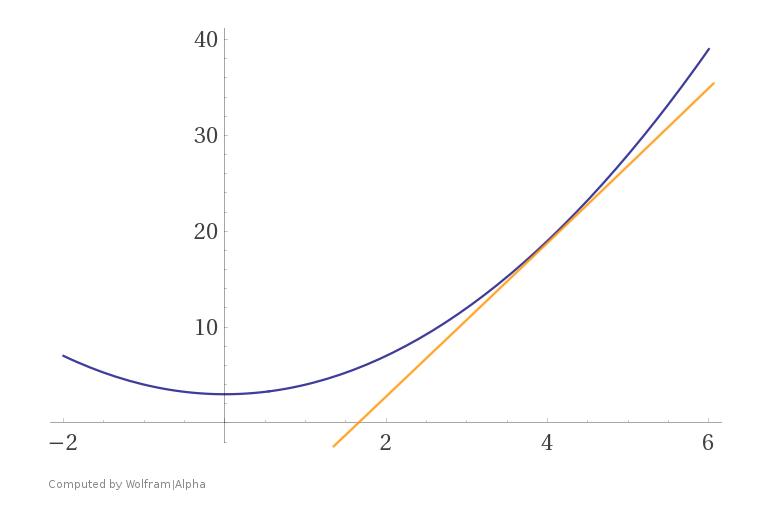
\includegraphics[width=2.5in]{WolframAlpha-yx21tangent4.png}
    \caption{$f(x) = x^2 + 1$, with tangent line on $f$ at $x=4$}
\end{figure}

}


\frame{ \frametitle{Derivative of a Real-Valued Function}

We may also be familiar with this definition written in the form 

\[ f'(x) = \lim_{\Delta x \to 0} \frac{f(x + \Delta x) - f(x)}{\Delta x} = \lim_{\Delta x \to 0} \frac{\Delta y}{\Delta x}  \]

\vspace{3mm}

where $y = f(x)$, and possibly using $h = \Delta x$. 

}


\frame{ \frametitle{Derivative of a Real-Valued Function}

Other notations for the derivative include 

\[ \frac{dy}{dx} = \frac{d}{dx} f(x) = y' = f'(x). \]

\vspace{3mm}

If $f'(c)$ exists for $c \in (a,b)$, we say $f$ is \textbf{differentiable} at $c$. 

\vspace{3mm}

If $f'(c)$ exists $\forall c \in S \subseteq (a,b)$, we say $f$ is \textbf{differentiable} on $S$. 


}


\frame{ \frametitle{Derivative of a Real-Valued Function}

Note that the derivative is a limit, meaning there are two one-sided limits that must match: the \textbf{one-sided derivatives} of $f$ at $c$ are 

\begin{align*} 
f'_-(x) & = \lim_{\Delta x \to 0-} \frac{f(x + \Delta x) - f(x)}{\Delta x}, \\
f'_+(x) & = \lim_{\Delta x \to 0+} \frac{f(x + \Delta x) - f(x)}{\Delta x}.
\end{align*} 

Thus, for $f'(x)$ to exist, we require $f'_-(x) = f'_+(x)$. 

\vspace{3mm}

In the case of endpoints of an interval, say, 

\[ f:[a,b] \to \R, \]

\vspace{3mm}

we only consider the one available direction, i.e. $f'_+(a)$ and $f'_-(b)$. 

} 


% eg
\frame{ \frametitle{Example: Basic Derivative}

\begin{ex}
A standard first derivative example is the derivative of a parabola. 
\end{ex}
Let $f(x) = x^2 +3x - 6$. Then 
\begin{align*} 
D_f(x,c) = \frac{f(x) - f(c)}{x - c} & = \frac{x^2 + 3x - 6 - c^2 - 3c + 6}{x-c} \\
 & = \frac{x^2- c^2 + 3(x-c)}{x-c} = x + c + 3 
\end{align*}
for $x \neq c$, which implies 
\[ f'(c) = \lim_{x \to c} (x + c + 3) = 2c + 3. \]

}


% sequential criterion for cont
\frame{ \frametitle{Sequential Criterion for Differentiability}

\begin{thm}
Let $f: (a,b) \to \R$ be a function, and $c \in (a,b)$. 

\vspace{3mm}

Then $f$ is differentiable at $c$ $\iff$ for every sequence $(x_n)$ in $(a,b)$ such that $x_n \to c$, we have 
\[ \lim_{n \to \infty} D_f(x_n, c) = \lim_{n \to \infty} \frac{f(x_n) - f(c)}{x_n - c} = L. \]
Then $L = f'(c)$. 
\end{thm}

\vspace{5mm}

This theorem is particularly useful in the contrapositive; \\to show that $f$ does not have a derivative at $c$, show 
\[ \exists \text{ a sequence } (x_n) \text{ converging to } c: \,\, D_f(x_n, c) \text{ does not have a limit.} \]

}


% eg, |x|
\frame{ \frametitle{Example: Absolute Value}

\begin{ex}
\[ f(x) = |x| = \left\{ \begin{array}{rl} x & x \geq 0 \\ -x & x < 0 \end{array} \right. \]
does not have a derivative at $x=0$: 
\end{ex}
\begin{align*} 
f'_-(0) & = \lim_{\Delta x \to 0-} \frac{f(0+\Delta x) - f(0)}{\Delta x} = -1 \\
f'_+(0) & = \lim_{\Delta x \to 0+} \frac{f(0+\Delta x) - f(0)}{\Delta x} = +1
\end{align*}
$f'_-(0) \neq f'_+(0)$. \,\,\,\, $\therefore f'(0)$ DNE. 

}


\frame{ \frametitle{Example: Absolute Value}

\begin{figure}[!ht]
  \centering
    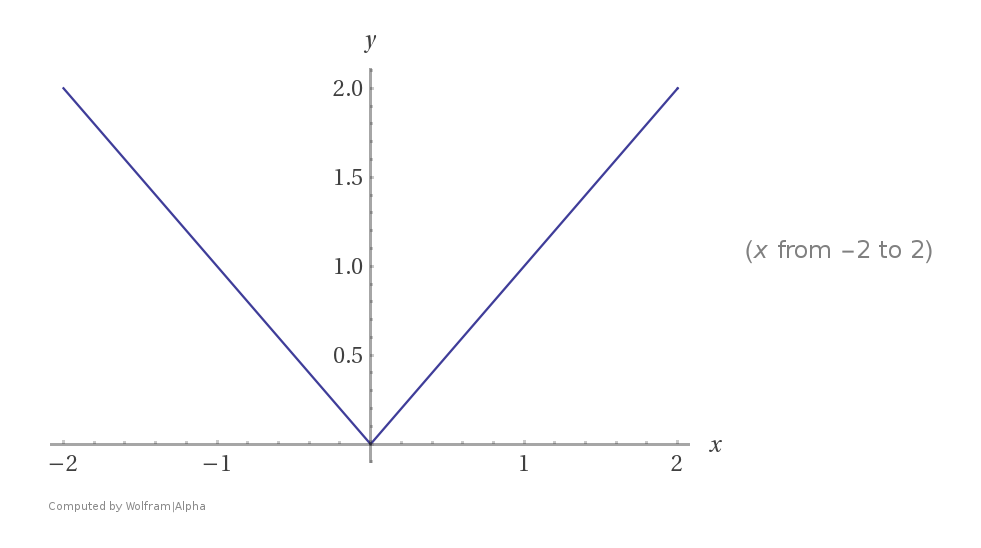
\includegraphics[width=4in]{yabsx.png}
    \caption{$f(x) = |x|$}
\end{figure}

}


% thm: f diff \implies f cont
\frame{ \frametitle{$f$ differentiable $\implies$ $f$ continuous}

Our next theorem relates differentiability and continuity: 

\vspace{5mm}

\begin{thm} 
A function $f$ is differentiable at $c$ $\implies$ $f$ is continuous at $c$. 
\end{thm}

}


\frame{ \frametitle{$f$ differentiable $\implies$ $f$ continuous}

\pf If $x \neq c$, 
\begin{align*} 
f(x) & = f(c) + f(x) - f(c) \\
 & = f(c) + \frac{f(x) - f(c)}{x - c}(x - c) = f(c) + D_f(x, c)(x - c).
\end{align*}

Thus, since $f$ is differentiable at $c$, 
\begin{align*} 
\lim_{x \to c} f(x) & =  \lim_{x \to c} \left[ f(c) + D_f(x, c)(x - c) \right] \\
 & = f(c) + \cancel{f'(c) (c - c)} = f(c). \,\, \blacksquare
\end{align*}
}



% thm: properties: linearity, product/quotient rules
\frame{ \frametitle{Basic Derivative Rules}

Consider $f$ and $g$ differentiable on $(a,b)$, and let $c_1, c_2 \in \R$. 

\vspace{3mm}

Recall some basic differentiation rules: 

\vspace{3mm}

\begin{itemize}
\item Differentiation is a \textbf{linear operation}: 
\[ \frac{d}{dx} \left( c_1 f(x) + c_2 g(x) \right) = c_1 f'(x) + c_2 g'(x). \]

\vspace{3mm}

\item \textbf{Product Rule}: 
\[ \frac{d}{dx} \left( f(x) g(x) \right) = f'(x) g(x) + f(x) g'(x). \]
\end{itemize}

}


\frame{ \frametitle{Basic Derivative Rules}

\begin{itemize}
\item \textbf{Chain Rule (Composition)}: If $(g \circ f)(x) = g(f(x))$, 
\[ \frac{d}{dx} \left( g(f(x)) \right) = g'(f(x)) f'(x). \]

\vspace{3mm}

\item \textbf{Quotient Rule}: if $g(x) \neq 0$, 
\[ \frac{d}{dx} \left( \frac{f(x)}{g(x)} \right) = \frac{f'(x) g(x) - f(x) g'(x)}{(g(x))^2}. \]
\end{itemize}

}

% eg: power rule ($\N$)
\frame{ \frametitle{Example: Power Rule $(\N)$}

\begin{prop}
Let $n \in \N$. Then the derivative of $f(x) = x^n$ is $f'(x) = nx^{n-1}$: 
\end{prop}

\vspace{3mm}

\pf 
\begin{align*}
D_f(x,c) & = \frac{x^n - c^n}{x - c} = \frac{(x-c)\left( \sum_{k=0}^{n-1} x^k c^{n-1-k}\right)}{x-c} = \sum_{k=0}^{n-1} x^k c^{n-1-k} \\
\implies f'(c) & = \lim_{x \to c} \sum_{k=0}^{n-1} x^k c^{n-1-k} = \sum_{k=0}^{n-1} \left( \lim_{x \to c} x^k \right) c^{n-1-k} \\
 & = \sum_{k=0}^{n-1} c^k c^{n-1-k} = \sum_{k=0}^{n-1} c^{n-1} = nc^{n-1}. \,\, \blacksquare
\end{align*}

(Another proof uses induction and the product rule.)

}


% thm: chain rule
\frame{ \frametitle{Chain Rule}

\begin{thm} % 1.11 Thm II
\textbf{(Chain Rule)} Let $f: I \to \R$ and $g: J \to \R$ be differentiable, and let the image $f(I) \subseteq J$. Then the composite function $g \circ f:I \to \R$,
\[ (g \circ f)(x) = g(f(x)), \]
 is differentiable, and  
\[ \frac{d}{dx}[g(f(x))] = g'(f(x)) f'(x). \]
\end{thm}
You may be familiar with the Leibniz notation for the chain rule: 
\[ y = g(u), \,\, u = f(x) \implies \frac{dy}{dx} = \frac{dy}{du} \cdot \frac{du}{dx}. \]

}


\frame{ \frametitle{Chain Rule}

\pf First, we'll construct the difference quotient $D_{g \circ f}$: 
\[ D_{g \circ f}(x, c) = \frac{g(f(x)) - g(f(c))}{x-c}. \]

\vspace{3mm}

Being careful to avoid a zero denominator, for $x \neq c$ such that $f(x) \neq f(c)$, we say 
\[ D_{g \circ f}(x, c) = \frac{g(f(x)) - g(f(c))}{f(x) - f(c)} \cdot \frac{f(x) - f(c)}{x-c}. \]

}


\frame{ \frametitle{Chain Rule}

Since we need to take a limit as $x \to c$, we cannot necessarily avoid the situation $f(x) = f(c)$, so we notice that  
\[ \lim_{y \to f(c)}  \frac{g(y) - g(f(c))}{y - f(c)} = g'(f(c)). \]

\vspace{3mm}

We define the function 
\[ h(y) = \left\{ \begin{array}{ll} \frac{g(y) - g(f(c))}{y - f(c)} = D_g(y, f(c)) & y \neq f(c) \\
g'(f(c)) & y = f(c), 
\end{array} \right. \]

\vspace{3mm}

and see that $h$ is continuous at $y = f(c)$ (by definition!). 

}


\frame{ \frametitle{Chain Rule}

$f$ is continuous at $c$, so since composition of continuous functions is continuous, 

\begin{align*} 
\lim_{y \to f(c)} \frac{g(y) - g(f(c))}{y - f(c)} = g'(f(c)) = h(f(c)) = \lim_{x \to c} h(f(x)).
\end{align*}

\vspace{3mm}

Next, note that if $x \in I$, then $y = f(x) \in J$. Since 
\[ g(y) - g(f(c)) = h(y) \cdot (y - f(c)) \]

\vspace{3mm}

for any $y \in J$, then for all $x \in I$, we have 
\[ g(f(x)) - g(f(c)) = h(f(x)) \cdot (f(x) - f(c)). \]

}



\frame{ \frametitle{Chain Rule}

Hence, for $x \in I$, $x \neq c$, we have 
\[ \frac{g(f(x)) - g(f(c))}{x-c} = h(f(x)) \cdot \frac{f(x) - f(c)}{x-c} = h(f(x)) \cdot D_f(x,c). \]

\vspace{3mm}

All this rearranging gets us the limit 
\begin{align*}
(g \circ f)'(x) & = \lim_{x \to c} D_{g \circ f}(x, c) \\
 & = \lim_{x \to c} h(f(x)) \cdot D_f(x,c) = g'(f(c)) \cdot f'(c). \,\, \blacksquare
\end{align*}

}


% The Mean Value Theorem

% thm: f diff on (a,b), f assumes max or min at c implies f'(c) = 0
\frame{ \frametitle{Relative/Absolute Extrema}

\begin{defn}
Let $f:D \to \R$ be a function, and $c \in D$.

\vspace{5mm}

We say $f$ has a \textbf{relative (local) maximum} at $c$ if 
\[ \exists h >0 \,\, \exists N(c,h): \,\, \forall x \in N(c,h), \,\, f(x) \leq f(c). \]

\vspace{3mm}

$f$ has a \textbf{relative (local) minimum} at $c$ if 
\[ \exists h >0 \,\, \exists N(c,h): \,\, \forall x \in N(c,h), \,\, f(x) \geq f(c). \]
\end{defn}

}


\frame{ \frametitle{Relative/Absolute Extrema}

The relative (local) maxima and minima of $f$ are called its 

\begin{center}
\textbf{relative (local) extrema}. 
\end{center}

\vspace{5mm}

Replacing the neighborhood $N$ with the full set $D$ results in the 

\begin{center}
\textbf{absolute (global) extrema}. 
\end{center}

of $f$.  

}


\frame{ \frametitle{Relative Extremum \& Differentiable $\implies$ Derivative Zero}

\begin{thm} 
If $f: (a,b) \to \R$ has a (relative) extremum at $c \in (a,b)$ 
and $f$ is differentiable, then $f'(c) = 0$. % critical point with a zero
\end{thm}

\vspace{5mm}

\pf WLOG say $f(c)$ is a relative maximum. Then 
\[ \exists \delta > 0: \,\, |x - c| < \delta \implies f(x) \leq f(c). \]

}


\frame{ \frametitle{Relative Extremum \& Differentiable $\implies$ Derivative Zero}

Hence, the one-sided derivatives of $f$ at $c$ are such that 

\begin{align*} 
(x < c) \,\,\,\, f'_-(c) & = \lim_{x \to c-} D_f(x, c) = \lim_{x \to c-} \frac{f(x) - f(c)}{x - c} \geq 0 \\
 & \\
(x > c) \,\,\,\, f'_+(c) & = \lim_{x \to c+} D_f(x, c) = \lim_{x \to c+} \frac{f(x) - f(c)}{x - c} \leq 0.
\end{align*}

\vspace{3mm}

If $f$ is differentiable at $c$, then 
\[ f'(c) = f'_-(c) = f'_+(c) \implies f'(c) = 0. \,\, \blacksquare \]

\vspace{5mm}

(Another proof uses sequences.)
}


\frame{ \frametitle{Relative Extremum $\cancel{\implies}$ Differentiable}

$f$ having a relative extremum at $c$ does not guarantee that $f$ is differentiable at $c$. 

\vspace{3mm}

It may be the case that $f'(c)$ does not exist. 

\vspace{3mm}

\begin{ex}
$f: \R \to \R$ defined by 
\[ f(x) = |x-4| \] 

is defined for all $x \in \R$, and has a relative minimum at $x=4$, \\but $f$ is not differentiable at $x=4$: 

\[ f'(x) = \left\{ \begin{array}{rl} 1 & x > 4 \\ -1 & x < 4 \\ DNE & x = 4 \end{array} \right. \]
\end{ex}

}



\frame{ \frametitle{Derivative Zero $\cancel{\implies}$ Relative Extremum}

It is also not true that $f'(c) = 0$ for some $c \in (a,b)$ means $f$ has a relative extremum at $c$. 

\vspace{3mm}

\begin{ex}
$f: \R \to \R$ defined by 
\[ f(x) = (x+6)^3 \] 
is defined for all $x \in \R$, and has $f(-6) = 0$ and $f'(-6) = 0$: 
\[ f'(x) = 3(x+6)^2. \]
However, in any neighborhood of $-6$, i.e. for any $\delta > 0$, 
\[ f(-6 - \delta) = -\delta^3 < 0, \,\, f(-6 + \delta) = \delta^3 > 0. \]
\end{ex}

$f'(c) = 0$ here is a \emph{necessary}, but not \emph{sufficient}, condition. 

}


\frame{ \frametitle{Rolle's Theorem}

\begin{thm}
\textbf{(Rolle's Theorem)} If $f:[a,b] \to \R$ is continuous on $[a,b]$ (one-sided at endpoints) and differentiable on $(a,b)$, then  \[ f(a) = f(b) \implies \exists c \in (a,b): \,\, f'(c) = 0. \]
\end{thm}

\vspace{3mm}

\pf If $\forall x \in [a,b]$, $f(x) = k$ for some constant $k$, this is obvious.

\vspace{3mm}

Thus, WLOG assume $\exists x_1, x_2 \in (a,b)$: $f(x_1) < f(x_2)$. 

}


\frame{ \frametitle{Rolle's Theorem}

$f$ is continuous on the closed interval $[a,b]$, and so by the EVT, attains its absolute maximum $M$ and minimum $m$.

\vspace{5mm}

Since $f(a) = f(b)$, and we assume $f(x) > f(a)$ for some $x \in (a,b)$. 

\vspace{5mm}

Since $f$ is differentiable on $(a,b)$, and 
\[ \exists c \in (a,b): \,\, f(c) = M, \text{ a maximum,} \] 

then by the previous theorem, $f'(c) = 0$.  $\blacksquare$ 

} 


% The Law of the Mean (MVT For Derivatives)
\frame{ \frametitle{Mean Value Theorem For Derivatives (Law of the Mean)}

\begin{thm}
\textbf{(Mean Value Theorem)} If $f:[a,b] \to \R$ is continuous on $[a,b]$ and is differentiable on $(a,b)$, then 
\[ \exists c \in (a,b): \,\, \frac{f(b) - f(a)}{b-a} = f'(c). \]
\end{thm}

} 


% The Law of the Mean (MVT For Derivatives)
\frame{ \frametitle{Mean Value Theorem For Derivatives (Law of the Mean)}

We interpret this fact geometrically as saying:

\vspace{3mm}
 
Any function differentiable on a closed interval $[a,b]$ 

\vspace{3mm}
 
contains a point whose  

\vspace{3mm}
 
derivative (tangent line slope, instantaneous rate of change) 

\vspace{3mm}
 
is equal to the 

\vspace{3mm}
 
average rate of change over the interval, 

\vspace{3mm}
 
i.e. the secant line slope between the endpoints of the interval.

}


\frame{ \frametitle{Mean Value Theorem For Derivatives (Law of the Mean)}

\begin{figure}[!ht]
  \centering
    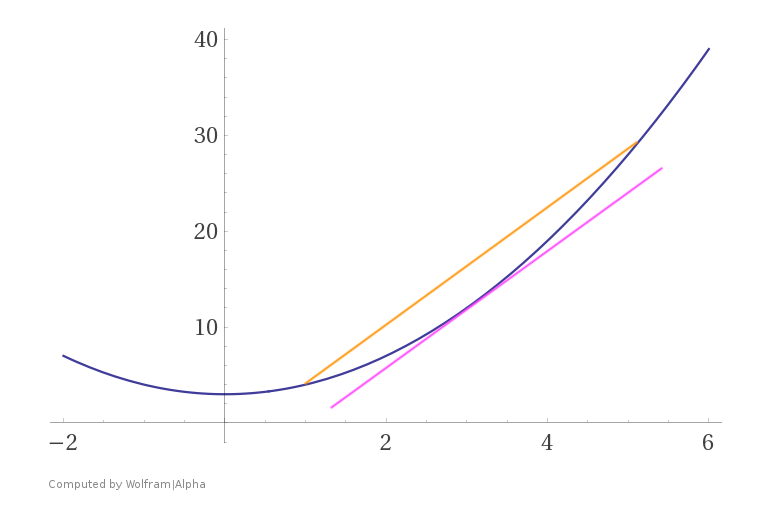
\includegraphics[width=3in]{WolframAlpha-yx21secant15tangentMVT.png}
    \caption{$f(x) = x^2 + 1$, with secant line between $x=1$ and $x=5$, and a parallel tangent line}
\end{figure}

}


\frame{ \frametitle{Proof of the Mean Value Theorem For Derivatives}

\pf \textbf{of MVT}: Define 
\[ h(x) = f(x) - f(a) - \left(\frac{f(b) - f(a)}{b-a}\right)(x-a). \]

Since $h$ is continuous on $[a,b]$ and differentiable on $(a,b)$, and 
\[ h(a) = h(b) = 0, \]
then by Rolle's Theorem 
\[ \exists c \in (a,b): \,\, h'(c) = 0. \]

But 
\[ h'(x) = f'(x) - \frac{f(b) - f(a)}{b-a}. \]

Therefore, 
\[ f'(c) = \frac{f(b) - f(a)}{b-a}. \,\, \blacksquare \]


}


% thm: f cont on [a,b], diff on (a,b), f'(x) = 0 \implies f(x) const on [a,b]
\frame{ \frametitle{Corollaries of the Mean Value Theorem For Derivatives}

Two corollaries of the MVT tell us, without needing integrals, that 

\begin{enumerate}
\item if $f'(x) = 0$, then $f$ is a constant; 
\item if $f'(x) = g'(x)$, then $f = g$ up to a constant.
\end{enumerate}

\vspace{5mm}

\begin{cor} 
If $f: [a,b] \to \R$ is differentiable on $(a,b)$, and 
\[ \forall x \in (a,b), \,\, f'(x) = 0, \] 

then $\exists c \in \R$ such that $f(x) = c$ for all $x \in [a,b]$ \\
(i.e. $f$ is constant on $[a,b]$). 
\end{cor}

}


\frame{ \frametitle{Corollaries of the Mean Value Theorem For Derivatives}

\pf For any $a \leq x_1 < x_2 \leq b$, the MVT hypotheses are satisfied, and so $\exists w \in (x_1, x_2)$:

\[ 0 = f'(w) = \frac{f(x_2) - f(x_1)}{x_2 - x_1} \implies f(x_1) = f(x_2). \]

\vspace{3mm}

But $x_1, x_2$ were chosen arbitrarily. $\therefore$ $f$ is constant $\forall a \leq x \leq b$. \,\, $\blacksquare$

}


\frame{ \frametitle{Corollaries of the Mean Value Theorem For Derivatives}

\begin{cor} 
If $f, g: [a,b] \to \R$ is differentiable on $(a,b)$, and 
\[ \forall x \in (a,b), \,\, f'(x) = g'(x), \]
 then 
\[ \exists C \in \R: \,\, \forall x \in [a,b], \,\, f(x) = g(x) + C. \]
\end{cor}

}


% defn: str inc/dec (monotone as well)
% thm: f'(x) > 0 implies str inc (likewise, <, str dec)
\frame{ \frametitle{Strictly, Monotone Increasing/Decreasing}

A function $f$ is \textbf{strictly (monotone) increasing} on an interval $I$ if 
\[ x_1 < x_2 \implies f(x_1) < f(x_2), \,\, (\leq) \]
and \textbf{strictly (monotone) decreasing} on $I$ if 
\[ x_1 < x_2 \implies f(x_1) > f(x_2), \,\, (\geq) \]

}


\frame{ \frametitle{Strictly, Monotone Increasing/Decreasing}

\begin{thm} Let $f$ be differentiable on an interval $I$. Then: 

$f'(x) > 0$ for all $x \in I$ $\implies$ $f$ is strictly increasing on $I$. \\
$f'(x) < 0$ for all $x \in I$ $\implies$ $f$ is strictly decreasing on $I$. \\
\end{thm}

\vspace{5mm}

\pf By the MVT, $\exists c \in (x_1, x_2) \subseteq I$ such that $x_1 < x_2$ and 
\[ f(x_2) - f(x_1) = f'(c)(x_2 - x_1). \]
Thus, $f(x_2) - f(x_1)$ and $f'(c)$ have the same sign. \,\, $\blacksquare$

}


% thm: IVT
\frame{ \frametitle{Intermediate Value Theorem (IVT) For Derivatives}

\begin{thm} 
\textbf{Intermediate Value Theorem (IVT)} Suppose $f$ is differentiable on $[a,b]$, and that $k$ is between $f'(a) \neq f'(b)$. Then 
\[ \exists c \in (a,b): \,\, f'(c) = k. \]
\end{thm}

\vspace{5mm}

\pf WLOG $f'(a) < k < f'(b)$. 

\vspace{5mm}

Let $g(x) = f(x) - kx$. Then $g$ is differentiable on $[a,b]$ and 
\[ g'(a) < 0 < g'(b). \]

}


\frame{ \frametitle{Intermediate Value Theorem (IVT) For Derivatives}
$g$ is continuous on $[a,b]$, which is compact, so $g$ assumes its minimum at some point $c \in [a,b]$. We need to show $c \in (a,b)$. 

\vspace{5mm}


Note that 
\begin{align*} 
g'(b) = \lim_{x \to b} \frac{g(x) - g(b)}{x-b} & = \lim_{x \to b} \frac{f(x) - f(b) - k(x-b)}{x-b} \\
 & \\
 & = f'(b) - k > 0,
\end{align*}
so there is a deleted neighborhood $U$ near $b$ such that 
\[ \forall x \in U \cap [a,b], \,\, \frac{g(x) - g(b)}{x-b} > 0. \] 

}


\frame{ \frametitle{Intermediate Value Theorem (IVT) For Derivatives}

Thus, for $x \in U \cap [a,b]$, if $x < b$, we must have $g(x) < g(b)$. 

\vspace{5mm}

Hence, $g(b)$ is not the minimum of $g$ on $[a,b]$, so $c \neq b$. 

\vspace{5mm}

Likewise, since $g'(a) < 0$, a similar argument shows that $c \neq a$. 

\vspace{5mm}

Therefore $c \in (a,b)$, and so by Rolle's Theorem, $g'(c) = 0$. 

\vspace{5mm}

Hence, 
\[ f'(c) = g'(c) + k = k. \,\, \blacksquare \]

}

% thm: inverse function thm
\frame{ \frametitle{Inverse Function Theorem}

\begin{thm}
\textbf{(Inverse Function Theorem, Derivatives)} 

\vspace{3mm}

Suppose that $f$ is differentiable on an interval $I$ and 
\[ \forall x \in I, \,\, f'(x) \neq 0. \] 

Then $f$ is injective, $f^{-1}$ is differentiable on $f(I)$, and  
\[ y = f(x) \implies (f^{-1})'(y) = \frac{1}{f'(x)}. \]
\end{thm}

}


\frame{ \frametitle{Proof of Inverse Function Theorem}

\pf $\forall x \in I$, $f'(x) \neq 0$, so $f'(x)$ must be the same sign $\forall x \in I$. 

\vspace{5mm}

WLOG say $f'(x) > 0$. 

\vspace{5mm}

Thus, $f$ is strictly increasing. Hence, $f$ is injective (and so the inverse function $f^{-1}$ exists). 

}


\frame{ \frametitle{Proof of Inverse Function Theorem}

Next, we show $f^{-1}$ is differentiable on $f(I)$. 

\vspace{5mm}

Let $y \in f(I)$ and let $(y_n)$ be any sequence in $f(I) \setminus \{y\}$ such that 
\[ y_n \to y. \] 

Then 
\[ x = f^{-1}(y) \] 

and, since $f^{-1}$ is continuous and injective, 
\[ (x_n = f^{-1}(y_n)) \] 

is a sequence in $I \setminus \{x\}$ converging to $x$. 

}


\frame{ \frametitle{Proof of Inverse Function Theorem}

$f'(x) \neq 0$ for all $x \in (a,b)$, so 
\[ \lim_{n \to \infty} \frac{f(x_n) - f(x)}{x_n - x} = f'(x) \neq 0. \]

\vspace{3mm}

Taking reciprocals and translating $x$ values into $y$ values, 
\begin{align*} 
\frac{1}{f'(x)} & = \lim_{n \to \infty} \frac{x_n - x}{f(x_n) - f(x)} \\
 & \\
  & = \lim_{n \to \infty} \frac{f^{-1}(y_n) -f^{-1}(y)}{y_n - y} = (f^{-1})'(y). \,\, \blacksquare
\end{align*}

}



% defn: indeterminate form: 
% $\frac{0}{0}$, $\frac{\infty}{\infty}$, $0 \cdot \infty$, $\infty^0$, $\infty - \infty$, ...
\frame{ \frametitle{Indeterminate Forms}

\begin{defn}
Suppose $f:D \to \R$ and $g:D \to \R$ are functions, and $c \in D$. If 
\[ \lim_{x \to c} f(x) = L \text{ and } \lim_{x \to c} g(x) = M, \]

with $L = M = 0$, then the limit 
\[ \lim_{x \to c} \frac{f(x)}{g(x)} \]

is called an \textbf{indeterminate form}. 
\end{defn}

\vspace{3mm}

A shorthand notation for this form is ``$\frac{0}{0}$''.

}


\frame{ \frametitle{Indeterminate Forms}

There are other indeterminate forms, such as 
\begin{itemize}
\item $0 \cdot \infty$, 
\item $\frac{\infty}{\infty}$, 
\item $\infty^0$, 
\item $0^0$, 
\item $1^{\infty}$, 
\item $\infty - \infty$, 
%\[ 0 \cdot \infty, \frac{\infty}{\infty}, \infty^0, 0^0, 1^{\infty}, \infty - \infty, \] 
\end{itemize}
that can be rewritten into $\frac{0}{0}$ form.

\vspace{5mm}

\textbf{L'H\^{o}pital's Rule} is a calculus-based way to evaluate such forms. 

}


% thm: Cauchy MVT
% 4.1 Cauchy's Generalized Law of the Mean
%\frame{ \frametitle{Cauchy's Generalized Law of the Mean (MVT)}
\frame{ \frametitle{Cauchy MVT (Generalized Law of the Mean)}

\begin{thm}
\textbf{(Cauchy Mean Value Theorem)} 

\vspace{3mm}

Suppose $f$ and $g$ are continuous on $[a,b]$ and differentiable on $(a,b)$. 
Then $\exists c \in (a,b)$ such that 
\[ [f(b) - f(a)] \, g'(c) = [g(b) - g(a)] \, f'(c). \]
\end{thm}

\begin{notenote}
If $g(x) = x$, then this reduces to the usual MVT: 
\[ \frac{f(b) - f(a)}{b-a} = f'(c). \]
\end{notenote}

}


\frame{ \frametitle{Cauchy MVT (Generalized Law of the Mean)}

\pf Let 
\[ h(x) = [f(b) - f(a)] \, g(x) - [g(b) - g(a)] \, f(x). \]

\vspace{3mm}

Then $h$ is continuous on $[a,b]$ and differentiable on $(a,b)$, and 
\[ h(a) = f(b)g(a) - g(b)f(a) = h(b). \]

\vspace{3mm}

By the MVT, $\exists c \in (a,b)$ such that $h'(c) = 0$. Hence, 
\[ [f(b) - f(a)] \, g'(c) = [g(b) - g(a)] \, f'(c). \,\, \blacksquare \]

}


% l'Hopital
\frame{ \frametitle{L'H\^opital's Rule}
%\frame{ \frametitle{L'Hospital's Rule}

\begin{thm} 
\textbf{(L'H\^{o}pital's Rule)} 

\vspace{3mm}

Suppose $f$, $g$ are continuous on $[a,b]$ and differentiable on $(a,b)$. 

\vspace{3mm}

Suppose $c \in [a,b]$ such that $f(c) = g(c) = 0$, and that 
\[ \exists \delta > 0: \,\, \forall x \in U = (a,b) \cap N^*(c, \delta), \,\, g'(x) \neq 0. \]

\vspace{3mm}

Then 
\[ \lim_{x \to c} \frac{f'(x)}{g'(x)} = L \in \R \implies \lim_{x \to c} \frac{f(x)}{g(x)} = L. \]
\end{thm}

}


\frame{ \frametitle{L'H\^opital's Rule}

\pf Let $(x_n)$ be a sequence in $U$ such that $x_n \to c$ and $x_n \neq c$.

\vspace{5mm}

For each $n \in \N$, let 
\[ a_n = \min(x_n, c) \text{ and } b_n = \max(x_n, c). \]

\vspace{3mm}

Then, by the Cauchy MVT on $f$ and $g$ on the intervals $[a_n, b_n]$, there exists sequence $(c_n)$ with $a_n < c_n < b_n$ such that 
\[ [f(x_n) - f(c)] \, g'(c_n) = [g(x_n) - g(c)] \, f'(c_n). \]

\vspace{3mm}

$g'(x) \neq 0$ for all $x \in U$, and $g(c) = 0$, so by the contrapositive of Rolle's Theorem, we have $g(x_n) \neq 0$ for all $n$. 

}


\frame{ \frametitle{L'H\^opital's Rule}

Since $f(c) = g(c) = 0$, we have $\forall n \in \N$, 
\[ f(x_n) g'(c_n) = g(x_n) f'(c_n) \implies \frac{f'(c_n)}{g'(c_n)} = \frac{f(x_n)}{g(x_n)}. \]

\vspace{3mm}

$x_n \to c$ and $c_n$ is always between $x_n$ and $c$, so $c_n \to c$.\footnote{This is true by the \emph{squeeze}, or \emph{sandwich theorem}: if $a_n \leq c_n \leq b_n$ for all $n \in \N$, and $\lim_{n \to \infty} a_n = \lim_{n \to \infty} b_n = L$, then $\lim_{n \to \infty} c_n = L$.}

\vspace{3mm}

Thus, by the sequential criterion for limits, 
\[ \lim_{n \to \infty} \frac{f'(c_n)}{g'(c_n)} = \lim_{x \to c} \frac{f'(x)}{g'(x)} = L \implies \lim_{n \to \infty} \frac{f(x_n)}{g(x_n)} = \lim_{x \to c} \frac{f(x)}{g(x)} = L. \,\, \blacksquare \]

}


\frame{ \frametitle{Limits of Functions of a Real Variable at Infinity}

Assume $\exists a \in \R$ such that $(a, \infty) \subseteq D$, and suppose $f: D \to \R$. 

\vspace{5mm}

The \textbf{long-term} or \textbf{asymptotic} behavior of $f$, or, simply, the \textbf{limit} of $f$ as $x \to \infty$, is denoted by 
\[ \lim_{x \to \infty} f(x) \] 

(with obvious similar definition for $x \to -\infty$). 

}


\frame{ \frametitle{Limits of Functions of a Real Variable at Infinity}

If the limit exists, i.e. $\exists L \in \R$ such that
\[ \forall \ve > 0, \,\, \exists M > 0: \,\, x > M \implies |f(x) - L| < \ve, \]

then we say 
\[ \lim_{x \to \infty} f(x) = L \] 

and that $f$ has a \textbf{horizontal asymptote} at $y = L$. 

}


\frame{ \frametitle{Limits of Functions of a Real Variable at Infinity}

Otherwise, if $f$ increases without bound, we say $f$ \textbf{tends to} $\infty$, and write 
\[ \lim_{x \to \infty} f(x) = \infty \]
if 
\[ \forall \alpha \in \R, \, \exists N = N(\alpha): \,\, x > N \implies f(x) > \alpha. \]

(We say f tends to $-\infty$ if $f$ decreases without bound). 

}


\frame{ \frametitle{L'H\^{o}pital's Rule (limit at $\infty$)}

\begin{thm} 
\textbf{(L'H\^opital's Rule, limit at $\infty$)} 

\vspace{3mm}

Suppose $f$ and $g$ are differentiable on $(a, \infty)$. Suppose also that 
\[ \lim_{x \to \infty} f(x) = \lim_{x \to \infty} g(x) = \infty, \]

\vspace{3mm}

and that $g'(x) \neq 0$ for $x \in (a, \infty)$. Then 
\[ \lim_{x \to \infty} \frac{f'(x)}{g'(x)} = L \in \R \implies \lim_{x \to \infty} \frac{f(x)}{g(x)} = L. \]

\end{thm}

}


\frame{ \frametitle{Higher-Order Derivatives}

If $f'$ is differentiable at $c$, then we call the \textbf{second derivative} of $f$ at $c$ the first derivative of $f'$ at $c$, denoted \[ f''(c) = (f')'(c). \] 

\vspace{3mm}

If $f''(c)$ exists, we say $f$ is \textbf{twice differentiable} at $c$. 

\vspace{5mm}

In general, if a function $f$ can be differentiated $n$ times on a domain $D$ (for $n \in \N$), we say $f$ has $n$th derivative 
\[ f^{(n)}(x) = (f^{(n-1)})'(x), \]

and if $f^{(n)}$ is continuous on $D$, we say that $f \in C^{n}(D)$.\footnote{We'll use the ``zeroth derivative" convention $f^{(0)}(x) = f(x)$.}

}


% thm: Taylor's Theorem (Lagrange)
\frame{ \frametitle{Taylor's Theorem (Lagrange)}

Taylor's Theorem generalizes the MVT for $n$th derivatives. 

\vspace{5mm}

\begin{thm} 
\textbf{(Taylor's Theorem)} 

\vspace{3mm}

Let $f \in C^{n+1}([a,b])$, and let $x_0 \in [a,b]$. 

\vspace{3mm}

Then, for each $x \in [a,b]$ with $x \neq x_0$, $\exists c$ between $x$ and $x_0$:
\begin{align*} 
f(x) = f(x_0) & + f'(x_0) (x-x_0) + \frac{f''(x_0)}{2!}(x-x_0)^2 \\
 & + ... + \frac{f^{(n)}(x_0)}{n!} (x-x_0)^n + \frac{f^{(n+1)}(c)}{(n+1)!} (x-x_0)^{n+1},  
\end{align*}
\end{thm}
where $n! = n(n-1)\cdots2\cdot 1$ for $n \in \N$ (``$n$ \textbf{factorial}'').\footnote{By convention, we define 0! = 1.}
}


% Taylor polynomials, remainder
\frame{ \frametitle{Taylor Polynomial, Remainder}

\begin{align*} 
f(x) = f(x_0) & + f'(x_0) (x-x_0) + \frac{f''(x_0)}{2!}(x-x_0)^2 \\
 & + ... + \frac{f^{(n)}(x_0)}{n!} (x-x_0)^n + \frac{f^{(n+1)}(c)}{(n+1)!} (x-x_0)^{n+1}  % + R_{n+1}, 
\end{align*}
has $n$th degree polynomial approximation 
\begin{align*} 
p_n(x) = f(x_0) & + f'(x_0) (x-x_0) + ... + \frac{f^{(n)}(x_0)}{n!} (x-x_0)^n, 
\end{align*}
called the \textbf{Taylor polynomial} of order $n$ of $f$ at $x_0$. Its error from $f(x)$ is the \textbf{remainder} term, for some $c \in (a,b)$, of  
\[ R_{n}(x) = f(x) - p_n(x) = \frac{f^{(n+1)}(c)}{(n+1)!} (x-x_0)^{n+1}. \]

}

\frame{ \frametitle{Taylor Series}

If $f \in C^{\infty}([a,b])$, i.e. $f$ is continuously differentiable infinitely many times, or \textbf{smooth}, on $[a,b]$, then the infinite sum produced by this method is called the \textbf{Taylor series} of $f$ at $x_0 \in [a,b]$: 

\[ f(x) = \sum_{n=0}^{\infty} \frac{f^{(n)}(x_0)}{n!} (x-x_0)^n. \]

}


\frame{ \frametitle{Taylor's Theorem (Lagrange)}

\pf \textbf{of Taylor's Theorem:} 

\vspace{3mm}

Fix $x \in [a,b]$ with $x \neq x_0$ and let $M$ be the unique solution of 
\begin{align} 
f(x) & = f(x_0) + f'(x_0) (x-x_0) \notag \\
 & + ... + \frac{f^{(n)}(x_0)}{n!} (x-x_0)^n + M(x-x_0)^{n+1}. \label{Taylor}
\end{align}
(This equation has a unique solution for $M$ because, with $x \neq x_0$, and $x$ and $x_0$ fixed, this is a linear equation in $M$.) 

\vspace{3mm}

We will prove that 
\[ M = \frac{f^{(n+1)}(c)}{(n+1)!} \] 
for some $c$ between $x$ and $x_0$. 

%\vspace{3mm}

}


\frame{ \frametitle{Taylor's Theorem (Lagrange)}

Define 
\begin{align*} 
F(t) = f(t) + f'(t) (x-t) + ... + \frac{f^{(n)}(t)}{n!} (x-t)^n + M(x-t)^{n+1}. 
\end{align*}
$F$ is a polynomial in $t$, and so is continuous on $[a,b]$ and differentiable on $(a,b)$. 

\vspace{3mm}

Since $a \leq x \leq b$ and $a \leq x_0 \leq b$, these results are also true for the interval between $x$ and $x_0$. 

}


\frame{ \frametitle{Taylor's Theorem (Lagrange)}

Next, note that 
\[ F(x) = f(x) \] 

since all but the first term cancel out, and 
\[ F(x_0) = f(x) \] 

since $M$ is the solution to \eqref{Taylor}. 

\vspace{3mm}

Thus, by the MVT, $\exists c$ between $x$ and $x_0$ such that 
\[ F'(c) = \frac{F(x) - F(x_0)}{x - x_0} = 0. \]

}


\frame{ \frametitle{Taylor's Theorem (Lagrange)}

Taking the derivative of $F(t)$, we see a telescoping sum (thanks to the product rule of differentiation): 
\begin{align*} 
F'(t) & = \left(f(t) + f'(t) (x-t) + ... + \frac{f^{(n)}(t)}{n!} (x-t)^n + M(x-t)^{n+1}\right)' \\
 & = {\color{blue} f'(t)} + {\color{red} f''(t) (x-t)} {\color{blue} - f'(t)} + ... \\
 & \,\,\,\,\, + {\color{orange}\frac{f^{(n)}(t)}{(n-1)!} (x-t)^{n-1}} {\color{brown}- \frac{f^{(n-1)}(t)}{(n-1)!}( -(n-1)(x-t)^{n-2})} \\
 & \,\,\,\,\, + \frac{f^{(n+1)}(t)}{n!} (x-t)^n {\color{orange} + \frac{f^{(n)}(t)}{n!} (-n(x-t)^{n-1})} \\
 & \,\,\,\,\,  - M(n+1)(x-t)^{n} \\
 & = \left[\frac{f^{(n+1)}(t)}{n!} - M(n+1)\right](x-t)^{n}.
\end{align*}


}


\frame{ \frametitle{Taylor's Theorem (Lagrange)}

Therefore, 
\begin{align*} 
F'(t) = \left[\frac{f^{(n+1)}(t)}{n!} - M(n+1)\right](x-t)^{n}
\end{align*}
and $F'(c) = 0$ implies 
\[ M = \frac{f^{(n+1)}(c)}{(n+1)!}. \,\,\,\, \blacksquare \]

}


\frame{ \frametitle{Taylor Series vs Power Series vs Generating Function}

A Taylor series is a type of a \textbf{power series}, which is an infinite-series representation of a function, in the form 
\[ f(x) = \sum_{n = 0}^{\infty} a_n x^n. \]

\vspace{3mm}

A power series of a function is a Taylor series around $x_0 = 0$, with coefficients 
\[ a_n = \frac{f^{(n)}(0)}{n!}. \]

}


\frame{ \frametitle{Taylor Series vs Power Series vs Generating Function}

All polynomials with degree $N$, for example, are power series such that $a_m = 0$ for all $m > N$ and $a_N \neq 0$.

\vspace{5mm}

A power series is a \textbf{generating function} that is also an actual function (not just a formal series).

\vspace{5mm}

Some functions  have infinitely many nonzero derivatives. 

}


\frame{ \frametitle{Taylor Series vs Power Series Example}

For example, consider the function 
\[ f(x) = 3x^2 - 5x + 7. \]

This function is a polynomial function, written in power series form: 
\[ f(x) = \sum_{n=0}^{\infty} a_n x^n; \,\,\,\, a_0 = 7, \,\, a_1 = -5, \,\, a_2 = 3, \,\, a_n = 0 \,\, \forall n > 2. \]

What is the Taylor series of $f$ at $x_0 = 2$?


}


\frame{ \frametitle{Taylor Series vs Power Series Example}

The Taylor series of $f$ centered at $x_0 = 2$ would have form 
\[ f(x) = \frac{f(2)}{0!} (x-2)^0 + \frac{f'(2)}{1!} (x-2)^1 + \frac{f''(2)}{2!} (x-2)^2 +  \frac{f''(3)}{3!} (x-2)^3 + ... \]

\vspace{5mm}

First, we can easily compute the derivatives of $f$: 
\[ f'(x) = 6x - 5, \,\, f''(x) = 6, \,\, f^{(n)}(x) = 0 \,\, \forall n > 2. \]

}


\frame{ \frametitle{Taylor Series vs Power Series Example}

Thus, we can limit ourselves to just the first three terms 
\[ f(x) = \frac{f(2)}{0!} (x-2)^0 + \frac{f'(2)}{1!} (x-2)^1 + \frac{f''(2)}{2!} (x-2)^2. \]

\vspace{5mm}

The values of derivatives of $f$ at $x_0 = 2$ are 
\[ f(2) = 9, \,\, f'(2) = 7, \,\, f''(2) = 6. \]

\vspace{5mm}

Thus, the Taylor series can be written 
\[ f(x) = 9 + 7(x-2) + 3(x-2)^2. \]
Simplifying this expression returns us to the Taylor series form 
\[ f(x) = 7 - 5x + 3x^2. \]

}


\frame{ \frametitle{Some Well-Known Taylor Series}

\begin{align*}
\frac{1}{1-x} & = \sum_{n=0}^{\infty} x^n & (\text{geometric series; } |x| < 1) \\
e^x & = \sum_{n=0}^{\infty} \frac{x^n}{n!} & (x \in \R) \\
\sin(x) & = \sum_{n=0}^{\infty} \frac{(-1)^n}{(2n+1)!} x^{2n+1} & (x \in \R) \\
\cos(x) & = \sum_{n=0}^{\infty} \frac{(-1)^n}{(2n)!} x^{2n} & (x \in \R) \\
\ln(1+x) & = \sum_{n=1}^{\infty} \frac{(-1)^{n+1}}{n} x^n & (x \in (-1, 1])
\end{align*}

}


\frame{ \frametitle{Taylor Approximations}

The \textbf{Taylor polynomials} of $f$ at $x_0$, 
\begin{align*} 
p_n(x) = f(x_0) & + f'(x_0) (x-x_0) + ... + \frac{f^{(n)}(x_0)}{n!} (x-x_0)^n, 
\end{align*}
can be used to approximate $f(x)$ close to $x_0$. 

\vspace{5mm}

We will revisit series in a later section.

}


\end{document}